% Generated by Sphinx.
\def\sphinxdocclass{report}
\documentclass[letterpaper,10pt,openany,oneside]{sphinxmanual}
\usepackage[utf8]{inputenc}
\DeclareUnicodeCharacter{00A0}{\nobreakspace}
\usepackage[T1]{fontenc}
\usepackage[english]{babel}
\usepackage{times}
\usepackage[Bjarne]{fncychap}
\usepackage{longtable}
\usepackage{sphinx}
\usepackage{multirow}


\title{Parallel Sorting}
\date{July 26, 2012}
\release{}
\author{CSInParallel Project}
\newcommand{\sphinxlogo}{}
\renewcommand{\releasename}{}
\makeindex

\makeatletter
\def\PYG@reset{\let\PYG@it=\relax \let\PYG@bf=\relax%
    \let\PYG@ul=\relax \let\PYG@tc=\relax%
    \let\PYG@bc=\relax \let\PYG@ff=\relax}
\def\PYG@tok#1{\csname PYG@tok@#1\endcsname}
\def\PYG@toks#1+{\ifx\relax#1\empty\else%
    \PYG@tok{#1}\expandafter\PYG@toks\fi}
\def\PYG@do#1{\PYG@bc{\PYG@tc{\PYG@ul{%
    \PYG@it{\PYG@bf{\PYG@ff{#1}}}}}}}
\def\PYG#1#2{\PYG@reset\PYG@toks#1+\relax+\PYG@do{#2}}

\def\PYG@tok@gd{\def\PYG@tc##1{\textcolor[rgb]{0.63,0.00,0.00}{##1}}}
\def\PYG@tok@gu{\let\PYG@bf=\textbf\def\PYG@tc##1{\textcolor[rgb]{0.50,0.00,0.50}{##1}}}
\def\PYG@tok@gt{\def\PYG@tc##1{\textcolor[rgb]{0.00,0.25,0.82}{##1}}}
\def\PYG@tok@gs{\let\PYG@bf=\textbf}
\def\PYG@tok@gr{\def\PYG@tc##1{\textcolor[rgb]{1.00,0.00,0.00}{##1}}}
\def\PYG@tok@cm{\let\PYG@it=\textit\def\PYG@tc##1{\textcolor[rgb]{0.25,0.50,0.56}{##1}}}
\def\PYG@tok@vg{\def\PYG@tc##1{\textcolor[rgb]{0.73,0.38,0.84}{##1}}}
\def\PYG@tok@m{\def\PYG@tc##1{\textcolor[rgb]{0.13,0.50,0.31}{##1}}}
\def\PYG@tok@mh{\def\PYG@tc##1{\textcolor[rgb]{0.13,0.50,0.31}{##1}}}
\def\PYG@tok@cs{\def\PYG@tc##1{\textcolor[rgb]{0.25,0.50,0.56}{##1}}\def\PYG@bc##1{\colorbox[rgb]{1.00,0.94,0.94}{##1}}}
\def\PYG@tok@ge{\let\PYG@it=\textit}
\def\PYG@tok@vc{\def\PYG@tc##1{\textcolor[rgb]{0.73,0.38,0.84}{##1}}}
\def\PYG@tok@il{\def\PYG@tc##1{\textcolor[rgb]{0.13,0.50,0.31}{##1}}}
\def\PYG@tok@go{\def\PYG@tc##1{\textcolor[rgb]{0.19,0.19,0.19}{##1}}}
\def\PYG@tok@cp{\def\PYG@tc##1{\textcolor[rgb]{0.00,0.44,0.13}{##1}}}
\def\PYG@tok@gi{\def\PYG@tc##1{\textcolor[rgb]{0.00,0.63,0.00}{##1}}}
\def\PYG@tok@gh{\let\PYG@bf=\textbf\def\PYG@tc##1{\textcolor[rgb]{0.00,0.00,0.50}{##1}}}
\def\PYG@tok@ni{\let\PYG@bf=\textbf\def\PYG@tc##1{\textcolor[rgb]{0.84,0.33,0.22}{##1}}}
\def\PYG@tok@nl{\let\PYG@bf=\textbf\def\PYG@tc##1{\textcolor[rgb]{0.00,0.13,0.44}{##1}}}
\def\PYG@tok@nn{\let\PYG@bf=\textbf\def\PYG@tc##1{\textcolor[rgb]{0.05,0.52,0.71}{##1}}}
\def\PYG@tok@no{\def\PYG@tc##1{\textcolor[rgb]{0.38,0.68,0.84}{##1}}}
\def\PYG@tok@na{\def\PYG@tc##1{\textcolor[rgb]{0.25,0.44,0.63}{##1}}}
\def\PYG@tok@nb{\def\PYG@tc##1{\textcolor[rgb]{0.00,0.44,0.13}{##1}}}
\def\PYG@tok@nc{\let\PYG@bf=\textbf\def\PYG@tc##1{\textcolor[rgb]{0.05,0.52,0.71}{##1}}}
\def\PYG@tok@nd{\let\PYG@bf=\textbf\def\PYG@tc##1{\textcolor[rgb]{0.33,0.33,0.33}{##1}}}
\def\PYG@tok@ne{\def\PYG@tc##1{\textcolor[rgb]{0.00,0.44,0.13}{##1}}}
\def\PYG@tok@nf{\def\PYG@tc##1{\textcolor[rgb]{0.02,0.16,0.49}{##1}}}
\def\PYG@tok@si{\let\PYG@it=\textit\def\PYG@tc##1{\textcolor[rgb]{0.44,0.63,0.82}{##1}}}
\def\PYG@tok@s2{\def\PYG@tc##1{\textcolor[rgb]{0.25,0.44,0.63}{##1}}}
\def\PYG@tok@vi{\def\PYG@tc##1{\textcolor[rgb]{0.73,0.38,0.84}{##1}}}
\def\PYG@tok@nt{\let\PYG@bf=\textbf\def\PYG@tc##1{\textcolor[rgb]{0.02,0.16,0.45}{##1}}}
\def\PYG@tok@nv{\def\PYG@tc##1{\textcolor[rgb]{0.73,0.38,0.84}{##1}}}
\def\PYG@tok@s1{\def\PYG@tc##1{\textcolor[rgb]{0.25,0.44,0.63}{##1}}}
\def\PYG@tok@gp{\let\PYG@bf=\textbf\def\PYG@tc##1{\textcolor[rgb]{0.78,0.36,0.04}{##1}}}
\def\PYG@tok@sh{\def\PYG@tc##1{\textcolor[rgb]{0.25,0.44,0.63}{##1}}}
\def\PYG@tok@ow{\let\PYG@bf=\textbf\def\PYG@tc##1{\textcolor[rgb]{0.00,0.44,0.13}{##1}}}
\def\PYG@tok@sx{\def\PYG@tc##1{\textcolor[rgb]{0.78,0.36,0.04}{##1}}}
\def\PYG@tok@bp{\def\PYG@tc##1{\textcolor[rgb]{0.00,0.44,0.13}{##1}}}
\def\PYG@tok@c1{\let\PYG@it=\textit\def\PYG@tc##1{\textcolor[rgb]{0.25,0.50,0.56}{##1}}}
\def\PYG@tok@kc{\let\PYG@bf=\textbf\def\PYG@tc##1{\textcolor[rgb]{0.00,0.44,0.13}{##1}}}
\def\PYG@tok@c{\let\PYG@it=\textit\def\PYG@tc##1{\textcolor[rgb]{0.25,0.50,0.56}{##1}}}
\def\PYG@tok@mf{\def\PYG@tc##1{\textcolor[rgb]{0.13,0.50,0.31}{##1}}}
\def\PYG@tok@err{\def\PYG@bc##1{\fcolorbox[rgb]{1.00,0.00,0.00}{1,1,1}{##1}}}
\def\PYG@tok@kd{\let\PYG@bf=\textbf\def\PYG@tc##1{\textcolor[rgb]{0.00,0.44,0.13}{##1}}}
\def\PYG@tok@ss{\def\PYG@tc##1{\textcolor[rgb]{0.32,0.47,0.09}{##1}}}
\def\PYG@tok@sr{\def\PYG@tc##1{\textcolor[rgb]{0.14,0.33,0.53}{##1}}}
\def\PYG@tok@mo{\def\PYG@tc##1{\textcolor[rgb]{0.13,0.50,0.31}{##1}}}
\def\PYG@tok@mi{\def\PYG@tc##1{\textcolor[rgb]{0.13,0.50,0.31}{##1}}}
\def\PYG@tok@kn{\let\PYG@bf=\textbf\def\PYG@tc##1{\textcolor[rgb]{0.00,0.44,0.13}{##1}}}
\def\PYG@tok@o{\def\PYG@tc##1{\textcolor[rgb]{0.40,0.40,0.40}{##1}}}
\def\PYG@tok@kr{\let\PYG@bf=\textbf\def\PYG@tc##1{\textcolor[rgb]{0.00,0.44,0.13}{##1}}}
\def\PYG@tok@s{\def\PYG@tc##1{\textcolor[rgb]{0.25,0.44,0.63}{##1}}}
\def\PYG@tok@kp{\def\PYG@tc##1{\textcolor[rgb]{0.00,0.44,0.13}{##1}}}
\def\PYG@tok@w{\def\PYG@tc##1{\textcolor[rgb]{0.73,0.73,0.73}{##1}}}
\def\PYG@tok@kt{\def\PYG@tc##1{\textcolor[rgb]{0.56,0.13,0.00}{##1}}}
\def\PYG@tok@sc{\def\PYG@tc##1{\textcolor[rgb]{0.25,0.44,0.63}{##1}}}
\def\PYG@tok@sb{\def\PYG@tc##1{\textcolor[rgb]{0.25,0.44,0.63}{##1}}}
\def\PYG@tok@k{\let\PYG@bf=\textbf\def\PYG@tc##1{\textcolor[rgb]{0.00,0.44,0.13}{##1}}}
\def\PYG@tok@se{\let\PYG@bf=\textbf\def\PYG@tc##1{\textcolor[rgb]{0.25,0.44,0.63}{##1}}}
\def\PYG@tok@sd{\let\PYG@it=\textit\def\PYG@tc##1{\textcolor[rgb]{0.25,0.44,0.63}{##1}}}

\def\PYGZbs{\char`\\}
\def\PYGZus{\char`\_}
\def\PYGZob{\char`\{}
\def\PYGZcb{\char`\}}
\def\PYGZca{\char`\^}
% for compatibility with earlier versions
\def\PYGZat{@}
\def\PYGZlb{[}
\def\PYGZrb{]}
\makeatother

\begin{document}

\maketitle
\tableofcontents
\phantomsection\label{index::doc}



\chapter{Parallel Machine Models}
\label{ParallelMachineModels/ParallelMachineModels::doc}\label{ParallelMachineModels/ParallelMachineModels:parallel-sorting}\label{ParallelMachineModels/ParallelMachineModels:parallel-machine-models}\setbox0\vbox{
\begin{minipage}{0.95\linewidth}
\textbf{For Students}

\medskip


You are likely reading this for an algorithms or data structures course, or perhaps some other course for a computer science (CS)  major.  Whether you choose to major in CS or are learning CS in the hopes of applying it to your chosen field, you should be aware that \textbf{the time of parallel computing is now}: all practitioners and theoreticians of computer science must be able to think in parallel when designing solutions to problems, because all computing platforms that we work on will be inherently parallel machines, in that they will contain multiple processing units capable of manipulating data simultaneously, i.e. \textbf{in parallel}.  For this reason, in this unit we will begin discussing the process of thinking in parallel when considering how to design algorithms to solve particular problems.  The first problem we will consider is one of the fundamental problems of computer science: that of sorting a set of N items, where N may be very large.  Before looking at parallel algorithms to solve this problem, we must first have a clear idea of what types of parallel platforms there are in practice and how we can use an abstract theoretical parallel machine instead to make it easier for us to reason about the complexity and performance of parallel algorithms.
\end{minipage}}
\begin{center}\setlength{\fboxsep}{5pt}\shadowbox{\box0}\end{center}
\setbox0\vbox{
\begin{minipage}{0.95\linewidth}
\textbf{For Instructors}

\medskip


This module is designed to be used when students are studying ‘divide and conquer’ sorting algorithms.  In particular, merge sort is used as an example.  This could be expanded to include quicksort and parallel implementations of it, such as that suggested by Quinn.
\end{minipage}}
\begin{center}\setlength{\fboxsep}{5pt}\shadowbox{\box0}\end{center}


\section{Learning Objectives}
\label{ParallelMachineModels/ParallelMachineModels:learning-objectives}

\subsection{Base Knowledge}
\label{ParallelMachineModels/ParallelMachineModels:base-knowledge}\begin{itemize}
\item {} 
Students should be able to describe the PRAM model of computation and how it differs from the classical RAM model.

\item {} 
Students should be able to describe the difference between the following memory access models associated with the PRAM model of computation: EREW, CREW, CRCW.

\item {} 
Students should be able to describe the difference between shred memory and distributed memory machine models.

\item {} 
Students should be able to visualize and describe these simple forms of communication interconnection between processors: linear array, mesh, binary tree.

\end{itemize}


\subsection{Conceptual/applied knowledge}
\label{ParallelMachineModels/ParallelMachineModels:conceptual-applied-knowledge}\begin{itemize}
\item {} \begin{description}
\item[{Given a theoretical PRAM shared memory model, a particular memory access model, and an interconnection network, students should be able to:}] \leavevmode\begin{itemize}
\item {} 
develop an algorithm for sorting a large collection of N data items,

\item {} 
develop an algorithm for searching a large collection of N data items {[}optional, future{]}

\item {} 
develop an algorithm for traversing a graph of size N {[}optional, future{]} and in all cases reason about the complexity of their solution.

\end{itemize}

\end{description}

\end{itemize}


\section{Perquisites and Assumed Level}
\label{ParallelMachineModels/ParallelMachineModels:perquisites-and-assumed-level}
Before studying this material, students should be familiar with the sequential version of merge sort, or at least some other type of divide and conquer recursive algorithm.  Students should also have an initial understanding of how to reason about time complexity of sorting algorithms in terms of the number of items being sorted. This reading assumes that the student may not be deeply familiar with computer organization and hardware yet, so these topics are approached in a relatively high-level, abstract way.
Models of Parallel Computatio


\section{Models of Parallel Computation}
\label{ParallelMachineModels/ParallelMachineModels:models-of-parallel-computation}

\subsection{Types of parallel computers, or platforms}
\label{ParallelMachineModels/ParallelMachineModels:types-of-parallel-computers-or-platforms}
Until 2004, when the first dual core processors for entry-level computer systems were sold, all computers that most individuals used on a regular basis contained one central processing unit (CPU).  These computers were classic von Neuman machines, where single instructions executed sequentially. Some of these instructions can read or write values to random access memory (RAM) connected to the CPU.  These machines are said to follow the traditional RAM model of computation, where a single processor has read and write (RW) access to memory.

Today, even the next generation of netbooks and mobile phones, along with our current laptops and desktop machines, have dual core processors, containing two ‘cores’ capable of executing instructions on one CPU chip.  High-end desktop workstations and servers now have chips with more cores (typicaly 4 or 8), which leads to the general term \emph{multicore} to refer to these types of CPUs.  This trend of increasing cores will continue for the foreseeable future- the era of single processors is gone.

In addition to the trend of individual machines containing multiple processing units, there is a growing trend towards harnessing the power of multiple machines together to solve ever larger computational and data processing problems.  Since the early to mid 1980’s, many expensive computers containing multiple processors were built to solve the world’s most challenging computational problems. Since the mid-1990’s, people have built clusters of commodity PCs that are networked together and act as a single computer with multiple processors (which could be multicore themselves). This type of cluster of computers is often referred to as a beowulf cluster, for the first of these that was built and published.  Major Internet software companies such as Google, Yahoo, and Microsoft now employ massive data centers containing thousands of computers to handle very large data processing tasks and search requests from millions of users.  Portions of these data centers can now be rented out at reasonable prices from Amazon Web Services, making it possible for those of us who can write parallel programs to harness the power of computers in ‘the cloud’- out on the Internet away from our own physical location.

Thus, in fairly common use today we have these major classes of parallel computing platforms:
\begin{itemize}
\item {} 
multicore with shared memory,

\item {} 
clusters of computers that can be used together, and

\item {} 
large data centers in the cloud.

\end{itemize}

In addition, in the past there were many types of multiprocessor computers built for parallel processing.  We draw on the research work conducted using these computers during the 1980’s and 1990’s to explain the following theoretical framework to describe models of parallel computing.


\subsection{Theoretical Parallel Computing Models}
\label{ParallelMachineModels/ParallelMachineModels:theoretical-parallel-computing-models}
The advent of these various types of computing platforms adds complexity to how we consider the operation of these machines.  For simplicity, we will loosely use the term \textbf{‘processor’} in the following discussion to refer to each possible processing unit that can execute instructions in the three major types of platforms described above (you will likely see this term being used differently in future hardware design or operating systems courses).  The memory might be shared by all processors, some of the processors, or none (each has its own assigned memory). Each processor may be capable of sending data to every other processor, but it may not.  We need to define a framework to describe these various possibilities as different types of computing models.  The type of computing model will dictate whether certain algorithms will be effective at speeding up an equivalent task on a single sequential  RAM computer.


\subsubsection{The PRAM Model}
\label{ParallelMachineModels/ParallelMachineModels:the-pram-model}
The sequential RAM computer with one processor differs from parallel computing platforms not only because there are multiple processing units, but also because they can vary in how available memory is accessed. When considering algorithms for parallel platforms, it is useful to consider an abstract, theoretically ideal computing model called a Parallel Random Access Machine, or PRAM. In such a machine, a single program runs on all processors, each of which has access to a main memory that is shared among them, as in Figure 1.
\begin{figure}[htbp]
\centering
\capstart

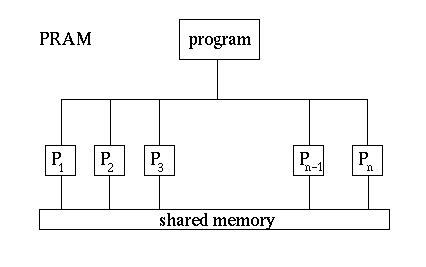
\includegraphics{Figure1.png}
\caption{\textbf{Figure 1}. The PRAM model. (Image taken from \href{http://www.mesham.com/article/Communication}{http://www.mesham.com/article/Communication})}\end{figure}

A PRAM machine with large numbers of processors has not been built in practice, but the model is useful when designing algorithms because we can reason about the complexity of those algorithms.  The common multicore machines available today can be considered to be PRAM, but have a low number of processors (n in Figure 1).  Note that the hardware involved to enable all processors to have access to memory is difficult to build so that it is fast, which is why we don’t yet have PRAM machines with many processors and large amounts of memory (This will be clearer when you’ve take a hardware design or computer organization course.)

Having many processing units, each running a program simultaneously, increases the complexity about how they coordinate to access memory. In this case, more than one processor may want to read from or write to the same memory location at the same time.  In the theoretical PRAM model, it is useful for us to consider the following three possible strategies for handling these simultaneous attempts to access a data element in memory:
\begin{enumerate}
\item {} 
Exclusive Read, Exclusive Write (\textbf{EREW}).  Only one processor at a time can read a memory value and only one processor at a time can write a memory value.

\item {} 
Concurrent Read, Exclusive Write (\textbf{CREW}).  Many processors can read a data value at one time, but only one processor at a time can write a memory value.

\item {} 
Concurrent Read, Concurrent Write (\textbf{CRCW}).  Many processors can read a data value at one time, and many processors can write a data value at one time.

\end{enumerate}

You may be wondering what we mean by a memory value.  We could consider various granularities: it might be a whole array of data, such as integers, or it might be the individual integers themselves.  In practice, this can vary for various types of hardware.  For simplicity, we will assume that one memory value is one data value, such as an integer, a floating point number, or a character- these are what each processor can access.

With each of these memory access models, we also need to consider what order the reads and writes will occur in. As you consider parallel algorithms for various tasks, it may become necessary to reason about which process of the more than one that require access to a data item will be chosen to go first. You want avoid solutions where the order of reads and writes will make a difference in the final result, but it may become important to specify ordering.
\begin{description}
\item[{\index{Concurrent Reads (CR)|textbf}Concurrent Reads (CR)}] \leavevmode\phantomsection\label{ParallelMachineModels/ParallelMachineModels:term-concurrent-reads-cr}
For concurrent reads (CR) between processors, all will get the same result and memory is not changed, so there is not a conflict at that single step that would cause your solution to be incorrect, unless you’ve devised an incorrect solution.

\end{description}
\begin{description}
\item[{\index{Exclusive Write (EW)|textbf}Exclusive Write (EW)}] \leavevmode\phantomsection\label{ParallelMachineModels/ParallelMachineModels:term-exclusive-write-ew}
Exclusive write (EW) typically means that your code should be designed so that only one processor is writing a data value to one memory location at one execution step.

\end{description}
\begin{description}
\item[{\index{Exclusive Read (ER)|textbf}Exclusive Read (ER)}] \leavevmode\phantomsection\label{ParallelMachineModels/ParallelMachineModels:term-exclusive-read-er}
Exclusive read (ER) usually means that your code should be written such that only one processor reads a data value at one step.

\end{description}

\begin{notice}{warning}{Warning:}
For EW and ER, a runtime error in your code would result if more than one processor attempted to read or write to the same data value at a certain step.
\end{notice}
\begin{description}
\item[{\index{Concurrent Writes (CW)|textbf}Concurrent Writes (CW)}] \leavevmode\phantomsection\label{ParallelMachineModels/ParallelMachineModels:term-concurrent-writes-cw}
Concurrent writes could be handled in a variety of ways; one of the more common approaches is to state that a higher (or lower) processor number goes first, thus giving it priority.  This concurrent write case is the hardest to design algorithms for.  Luckily, it is not yet achieved in practice, so we won’t spend time considering it.

\end{description}

All of this discussion about the PRAM model of a parallel machine leads us to one more important point that you may be wondering about: when we have a program running on multiple processors, just which step is running on each processor at any point in time? As you might guess, the answer once again in practice depends on the type of machine.  In the PRAM model we have two main types of program step execution on data:
\begin{itemize}
\item {} 
Multiple Instruction, Multiple Data (MIMD): each processor is stepping through the program instructions independently of the other processors, and each could be working on different data values.

\item {} 
Single Instruction, Multiple Data (SIMD): each processor is on the same instruction at any time, but but each is working on a separate data value.

\end{itemize}

For the rest of this discussion, we will assume that our PRAM machine is a MIMD machine.
\setbox0\vbox{
\begin{minipage}{0.95\linewidth}
\textbf{Stop and Consider this:}

\medskip


If we are assuming a SIMD PRAM machine, do we need to worry about which data access pattern (EREW, CREW, or CRCW) we have?
\end{minipage}}
\begin{center}\setlength{\fboxsep}{5pt}\shadowbox{\box0}\end{center}


\subsubsection{The distributed memory model}
\label{ParallelMachineModels/ParallelMachineModels:the-distributed-memory-model}
On the opposite extreme of the shared memory PRAM model is the the fully distributed model, as shown in Figure 2.  Here each processor has its own memory, and must communicate with other processors to share data.  Clusters and data centers fall into this category.  One of the common types of program execution models for the distributed memory case is called Single Program, Multiple Data (SPMD).  In SPMD, a program is written as a task to be executed on a portion of data, and each processor runs that program.  The data each processor works on may be sent to it from another processor, or may reside on it already.  At certain points in time, it may be necessary for the programs to synchronize and send each other data they have worked on.

Other hybrid parallel computer organizations have been built, in which processors have individual memory and a pool of shared memory.
\begin{figure}[htbp]
\centering
\capstart

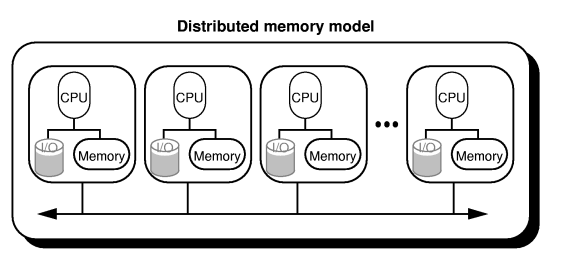
\includegraphics{Figure2.png}
\caption{\textbf{Figure 2} The fully distributed model. (Image take from \href{http://www.mesham.com/article/Communication}{http://www.mesham.com/article/Communication})}\end{figure}

The range of parallel computing platforms leads to a wide range of different programming models that are suited to a particular platform.  For the purposes of considering parallel algorithms and reasoning about their efficiency, however, it is useful to consider the theoretical PRAM model (MIMD assumed) with one of its 3 possible memory access strategies.  Thus, we can design algorithms and have a sense for how they will perform, and in practice will implement them using various platforms and associated software.


\subsubsection{Arrangement of Processors}
\label{ParallelMachineModels/ParallelMachineModels:arrangement-of-processors}
To design a parallel algorithm, we will assume PRAM as our base model. We will design a possible parallel solution, often by considering an original sequential solution and looking for places where operations can be run in parallel. Then we will examine whether the algorithm follows EREW, CREW, or CRCW access to data.  We may choose to fix the number of processors, \emph{n}, or we might begin with the simplified case of assuming we have an infinite number of processors. It will also be useful to consider a possible pattern of communication among the processors, which we can visualize as placing them in a particular arrangement.  The simplest arrangements are shown in Figure 3: a linear array (which can be extended to a ring by connecting P1 to Pn), a mesh, or a binary tree.
\begin{figure}[htbp]
\centering
\capstart

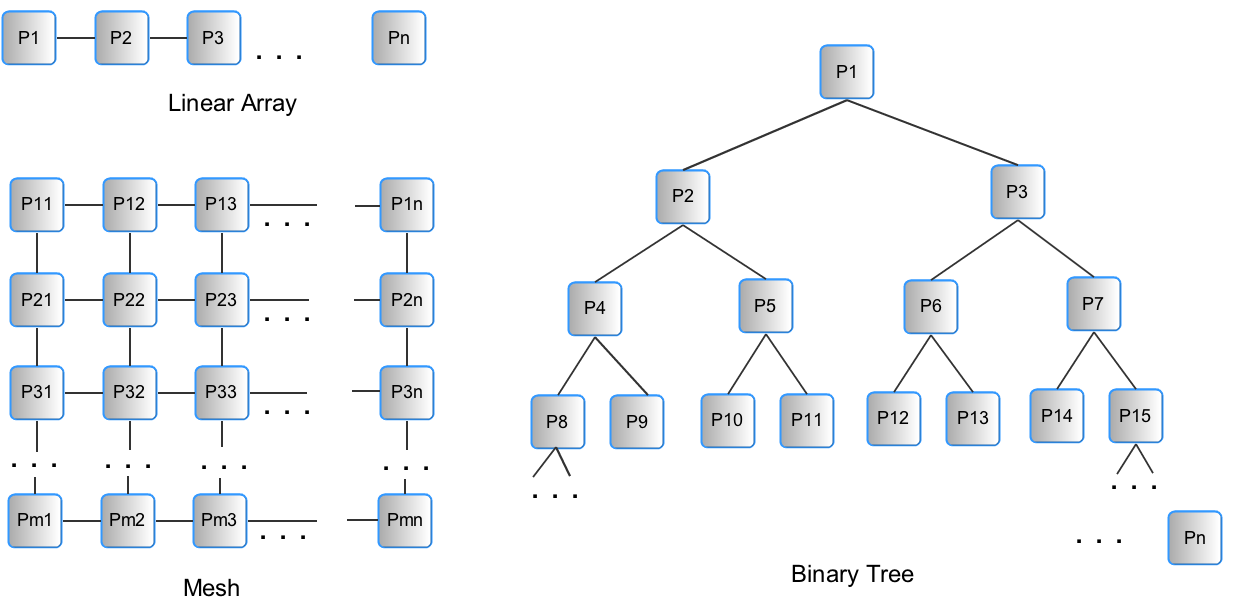
\includegraphics{Figure3.png}
\caption{\textbf{Figure 3} Simple, yet useful arrangements of processors to consider when designing parallel algorithms.}\end{figure}


\chapter{Parallel Merge Sort}
\label{MergeSort/MergeSort:parallel-merge-sort}\label{MergeSort/MergeSort::doc}

\section{The classic sequential version}
\label{MergeSort/MergeSort:the-classic-sequential-version}
This text assumes that you have studied the classical sequential RAM version of the famous recursive divide-and-conquer strategy for sorting N items called merge sort, which was first suggested by John von Neumann in 1945.  Please refer to your textbook or this source on wikipedia for details:  \href{http://en.wikipedia.org/wiki/Merge\_sort}{http://en.wikipedia.org/wiki/Merge\_sort} .  What follows is a brief reminder.

A pseudocode description for sequential merge sort is as follows, using two functions (taken from \href{http://www.codecodex.com/wiki/Merge\_sort}{http://www.codecodex.com/wiki/Merge\_sort}, which also contains implementations in several languages).  The \textbf{input} is an unsorted sequence of items (for simplicity, let’s assume integers). In the following code, this sequence of items could be an array of N items called m.  If N is extremely large, it is possible that m is a file on disk that is being read as a ‘stream’ (this is done for database systems, for example).
\setbox0\vbox{
\begin{minipage}{0.95\linewidth}
\textbf{code block}

\medskip


\begin{DUlineblock}{0em}
\item[] \textbf{function} mergesort(m)
\item[]
\begin{DUlineblock}{\DUlineblockindent}
\item[] \textbf{var} \emph{list} left, right
\item[] \textbf{if} length(m) $\le$ 1
\item[]
\begin{DUlineblock}{\DUlineblockindent}
\item[] \textbf{return} m
\end{DUlineblock}
\item[] \textbf{else}
\item[]
\begin{DUlineblock}{\DUlineblockindent}
\item[] middle = length(m) / 2
\item[] \textbf{for} \textbf{each} x \textbf{in} m \textbf{up} \textbf{to} middle
\item[]
\begin{DUlineblock}{\DUlineblockindent}
\item[] add x to left
\end{DUlineblock}
\item[] \textbf{for} \textbf{each} x \textbf{in} m \textbf{after} middle
\item[]
\begin{DUlineblock}{\DUlineblockindent}
\item[] add x to right
\end{DUlineblock}
\item[] left = mergesort(left)
\item[] right = mergesort(right)
\item[] result = merge(left, right)
\item[] \textbf{return} result
\end{DUlineblock}
\end{DUlineblock}
\end{DUlineblock}
\end{minipage}}
\begin{center}\setlength{\fboxsep}{5pt}\shadowbox{\box0}\end{center}
\setbox0\vbox{
\begin{minipage}{0.95\linewidth}
\textbf{code block}

\medskip


\begin{DUlineblock}{0em}
\item[] \textbf{function} merge(left,right)
\item[]
\begin{DUlineblock}{\DUlineblockindent}
\item[] \textbf{var} \emph{list} result
\item[] \textbf{while} length(left) \textgreater{} 0 \textbf{and} length(right) \textgreater{} 0
\item[]
\begin{DUlineblock}{\DUlineblockindent}
\item[] \textbf{if} first(left) $\le$ first(right)
\item[]
\begin{DUlineblock}{\DUlineblockindent}
\item[] append first(left) to result
\item[] left = rest(left)
\end{DUlineblock}
\item[] \textbf{else}
\item[]
\begin{DUlineblock}{\DUlineblockindent}
\item[] append first(right) to result
\item[] right = rest(right)
\item[] add x to right
\end{DUlineblock}
\end{DUlineblock}
\item[] \textbf{if} length(left) \textgreater{} 0
\item[]
\begin{DUlineblock}{\DUlineblockindent}
\item[] append left to result
\end{DUlineblock}
\item[] \textbf{if} length(right) \textgreater{} 0
\item[]
\begin{DUlineblock}{\DUlineblockindent}
\item[] append right to result
\end{DUlineblock}
\item[] \textbf{return} result
\end{DUlineblock}
\end{DUlineblock}
\end{minipage}}
\begin{center}\setlength{\fboxsep}{5pt}\shadowbox{\box0}\end{center}

In this algorithm, the data is split in half in the mergesort function, which is then called again on each half. This is done recursively until the size of each ‘half’ is one, at which point the left and right halves are merged together in a sorted list using the merge function. As each recursive call to merge completes, more of the halves are merged in sorted order and stored in a new array called result.
\setbox0\vbox{
\begin{minipage}{0.95\linewidth}
\textbf{Review Question}

\medskip


before going on, stop and be able to answer this: what is the time complexity of running this classical recursive merge sort on N items?
\end{minipage}}
\begin{center}\setlength{\fboxsep}{5pt}\shadowbox{\box0}\end{center}


\section{Let’s consider parallel versions}
\label{MergeSort/MergeSort:lets-consider-parallel-versions}
Now suppose we wish to redesign merge sort to run on a parallel computing platform.  Just as it it useful for us to abstract away the details of a particular programming language and use pseudocode to describe an algorithm, it is going to simplify our design of a parallel merge sort algorithm to first consider its implementation on an abstract PRAM machine.  However, we will also consider the realities of practical platforms and discuss a likely version that would get implemented in practice.

\emph{The key to designing parallel algorithms is to find the operations that could be carried out simultaneously.} This sometimes means that we examine a known sequential algorithm and look for possible simultaneous operations.


\subsection{Case 1: Fine-grained Simple merge sort}
\label{MergeSort/MergeSort:case-1-fine-grained-simple-merge-sort}
Suppose we have a PRAM machine with \textbf{n} processors.  A theoretically possible case, but unlikely in practice, would be that that we would have plenty of processors, so that n \textgreater{}= N, the size of our data to be sorted. This relatively impractical case is referred to as fine-grained parallelism.  We’ll look at the more practical course-grained case (n \textless{}\textless{} N)  later, but the fine-grained case provides a useful starting point for eventually arriving at course-grained solutions.

Let’s try looking at the original algorithm for where we can execute operations simultaneously.  When thinking about the sequential merge sort algorithm, a helpful way to visualize what is happening and reason about its complexity is to look at its recursion tree.  For example, if there were 8 items to be sorted, Figure 4 shows the recursive calls to the mergesort function  as boxes, with the number of items each recursive call would be working on.  Note that the merge function is called on every node but the leaves of this tree, where the input m is a single element.
\begin{figure}[htbp]
\centering
\capstart

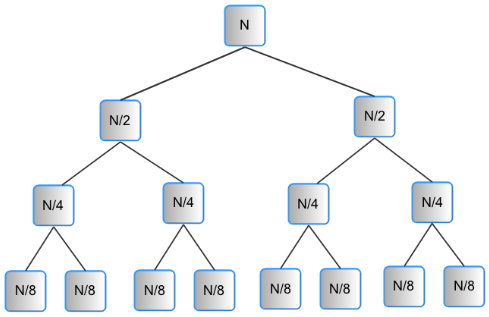
\includegraphics{Figure4.png}
\caption{\textbf{Figure 4}. A recursion tree for merge sort with N = 8 elements to be sorted.}\end{figure}

The sequential steps of this algorithm are taking place by following a depth-first traversal through this tree following the left children first. Take a moment to visualize, starting from the top node, which node begins executing the next mergesort function, and the next, and so on.  You might want to print Figure 4 and draw on it.

Now let’s examine which of these operations that were running one after the other in the sequential version could be run simultaneously on separate processors.  A natural way to split the work that can be run ‘in parallel’ is to do the work required at each level of the tree in Figure 4 simultaneously. Note that when considering a parallel solution, we use an \textbf{iterative approach} and envision starting our work at the bottom of the tree, moving up one level at each iteration. Each individual process is simply executing a merge on a range of values in the array (a single array could be used to sort in place, or a result could be used if you wish to preserve the original input).

Figure 5 shows an example of 8 elements to be sorted and what would result at each level of the tree.  At the level of the leaves of the tree, there is no real work, and we could begin by envisioning that level as our N data items, all shared in memory by our processors. At the next level, each of 4 processors can work on disjoint sets of 2 separate data items and merge them together. Once those are done, 2 processors can each work on merging to create a list of 4 sorted items, and finally, one last processor can merge those 2 lists of 4 to create the final list of 8 sorted items.  This becomes our parallel merge sort algorithm.
\begin{figure}[htbp]
\centering
\capstart

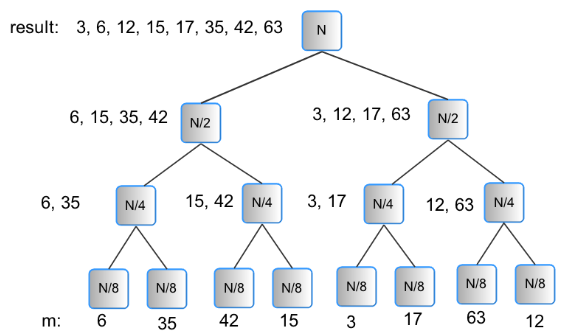
\includegraphics{Figure5.png}
\caption{\textbf{Figure 5}. An example of merge sorting a list of 8 integers.}\end{figure}

Because each processor executing in parallel at each level of the tree reads separate data items of the original input and writes to separate data items of the resulting output array in memory, we can consider this solution a EREW PRAM algorithm.
\setbox0\vbox{
\begin{minipage}{0.95\linewidth}
\textbf{in-class activity:}

\medskip


In class you will work on the pseudocode for this algorithm.
\end{minipage}}
\begin{center}\setlength{\fboxsep}{5pt}\shadowbox{\box0}\end{center}
\setbox0\vbox{
\begin{minipage}{0.95\linewidth}
\textbf{Algorithm Complexity:}

\medskip


After you consider the pseudocode solution, we will work through the complexity of this parallel approach.
\end{minipage}}
\begin{center}\setlength{\fboxsep}{5pt}\shadowbox{\box0}\end{center}


\subsection{Case 2: A scalable version of simple merge sort}
\label{MergeSort/MergeSort:case-2-a-scalable-version-of-simple-merge-sort}
The previous algorithm would not scale effectively for large sizes of N, because we would likely run out of processors.  Sorting is an often-run ‘benchmark test’ on very large parallel clusters, yet even then the number of processors is less than the number of data items, because the point of the benchmark is to run these sorting programs using very large numbers of data items to see how well the machine performs.  The previous algorithm, however, lets us understand the theoretical improvement that can be made when we employ multiple processors to solve the problem. Next let’s examine a more practical case.

We've established that the realistic case is when we have far fewer processors than the number of elements to be sorted. In this case, we need to have a strategy for separating the work to be done on each available processor.  We can start by deciding what a reasonable number of available processors is.  On multicore systems, the operating system itself may tell us just as we initiate the sort- in other words we would ask the OS for a set of processors.

A reasonable strategy is to still consider using a binary tree to illustrate the algorithm.  Given the number of processors to use, n,  we start by setting the number of leaf nodes of the tree to n.  For simplicity, it helps to imagine n as a power of 2, however, the algorithm will work with other values of n.  Each of the n nodes will first sort N/n of the original input data values, using a fast sequential sort mechianism, such as quicksort.  Two sorted lists can then be used by a `parent' process that will merge them.  That newly sorted list can be used by another parent process and merged with a second child sorted list. This process is repeated until the last two sublists get merged together.  Figure 6 shows how this algorithm wor\textbar{} Lend us a couple of bob till Thursday.
\begin{figure}[htbp]
\centering
\capstart

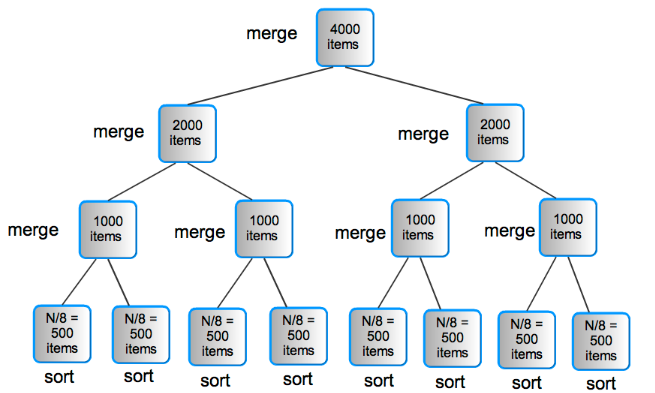
\includegraphics{Figure6.png}
\caption{\textbf{Figure 6}. Scaling parallel merge sort: an example where the number of data items, N is 4000 and the number of processors, n is 8.}\end{figure}
\setbox0\vbox{
\begin{minipage}{0.95\linewidth}
\textbf{Individual Activity:}

\medskip


Work through the complexity of this approach when using large values of N, where N is much greater than the number of processors.
\end{minipage}}
\begin{center}\setlength{\fboxsep}{5pt}\shadowbox{\box0}\end{center}


\chapter{In-class Slides and Activities}
\label{Slide/Slide:in-class-slides-and-activities}\label{Slide/Slide::doc}
The link below links to a slides which is designed for in-class activities. This slide will help you step through course materials as well as in-class activities.

\href{http://www.slideshare.net/sercuser/inclass-slides-with-activities}{http://www.slideshare.net/sercuser/inclass-slides-with-activities}


\chapter{Analysis of Parallel Merge Sort}
\label{AnalysisOfParallel/AnalysisOfParallel:analysis-of-parallel-merge-sort}\label{AnalysisOfParallel/AnalysisOfParallel::doc}
Here is the pseudocode for the Parallel Merge Sort algorithm, as we discussed in class (more or less):
\setbox0\vbox{
\begin{minipage}{0.95\linewidth}
\textbf{code block}

\medskip


\begin{DUlineblock}{0em}
\item[] PARALLEL MERGE SORT (A{[}0 . . . N - 1{]})
\item[]
\begin{DUlineblock}{\DUlineblockindent}
\item[] \textbf{set} s = 2
\item[] \textbf{while} s $\le$ N \textbf{do}
\item[]
\begin{DUlineblock}{\DUlineblockindent}
\item[] \textbf{do in parallel} with $\frac{N}{s}$ processors $p_i$
\item[]
\begin{DUlineblock}{\DUlineblockindent}
\item[] merge values from (s × i) to (s × i) + s - 1
\end{DUlineblock}
\item[] \textbf{set} s = 2 $\times$ s
\end{DUlineblock}
\end{DUlineblock}
\end{DUlineblock}
\end{minipage}}
\begin{center}\setlength{\fboxsep}{5pt}\shadowbox{\box0}\end{center}

We want to analyze the amount of work done by this algorithm, taking into account when things happen in parallel. We’ll use the input array size, \emph{N} , as the input size, and we’ll count the comparisons/copies done by the merge process as the basic operation. Because of the binary-tree structure of this algorithm, it makes sense to immediately apply a simplifying assumption, that the input size is a power of two:
\begin{gather}
\begin{split}N = 2^k\end{split}\notag
\end{gather}
The value of \emph{s} in the algorithm starts at 2, and goes up as a sequence of powers of two, stopping when it goes past $2^k$ . Thus, the \emph{while} loop will repeat \emph{k} times (try this out for $N = 2^6$ , for example).

Repeating \emph{k} times also means that the \emph{while} loop repeats $\log_2 N$ times, by the relationship between \emph{N} and \emph{k}.

Each pass through the \emph{while} loop, we have a set of merges that happen in parallel. In order to count the work done by merging on a particular pass, we count the cost of one merge of that size.

However, the amount of work done by a merge in the first pass through the \emph{while} loop is different from the amount of work done in the second pass, and so on. This is true because the size of the data being merged changes from one pass to another. Therefore we aren’t going to try to figure out a fixed amount of work within the \emph{while} loop, and then multiple by \emph{k}, the number of times the \emph{while} loop runs. That would overstate the work done. Instead, look at the amount of work per pass.

The first pass is always merging two values. We can call the work done there 2, as we have to copy both values to a new array and back again. On the second pass, each merge works on four data values: work done is therefore 4. The size of the data being merged doubles each time, and is a sequence of powers of two. Since the amount of work done by the merge is (roughly) equivalent to the size of the data, the work done starts at 2 and goes up as powers of two each pass.

So we can characterize the overall work done by the algorithm by the following summation. The bounds of the summation reflect the number of times the \emph{while} loop runs, and the body of the summation reflects the work done for one merge for that pass:
\begin{gather}
\begin{split}\sum_{i=1}^{k}2^i\end{split}\notag
\end{gather}
We can solve this summation as follows:
\begin{gather}
\begin{split}\sum_{i=1}^{k}2^i = (\sum_{i=0}^{k}2^i) - 1 \\
\sum_{i=1}^{k}2^i = (2^{k+1} - 1) - 1 \\
\sum_{i=1}^{k}2^i = (2 \cdot 2^k -2) \\
\sum_{i=1}^{k}2^i = 2n-2 \\\end{split}\notag
\end{gather}
This shows that the overall work done by Parallel Merge Sort is $O(n)$



\renewcommand{\indexname}{Index}
\printindex
\end{document}
